\documentclass{beamer}
\input{themes/packages.tex}
\usetheme{apertus}

\title{AXIOM Beta Main Board \\ and AXIOM Remote} 
\titlegraphic{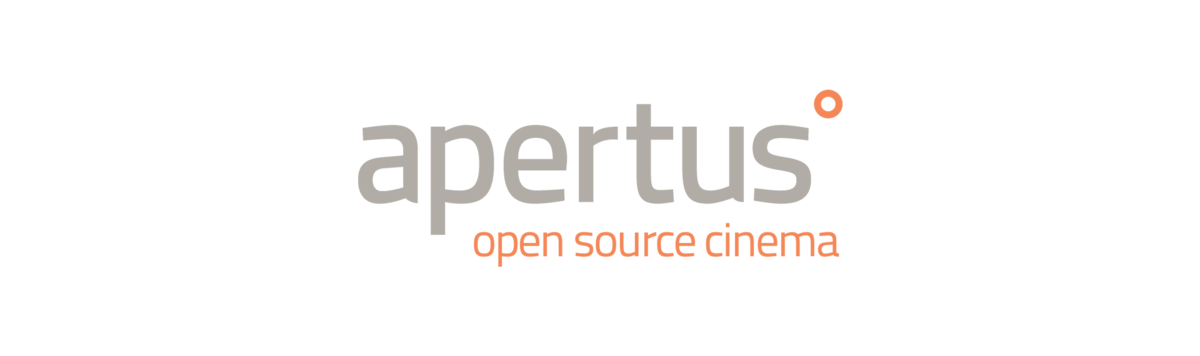
\includegraphics[width=10cm]{images/apertus_logo.png}}
\author{Ashok Singh \\ Priya Pandya \\ Swaraj Hota}
\date

\begin{document}
{
    \setbeamertemplate{footline}{} 
    \frame{\titlepage}
}

\section*{Outline}

\begin{frame}{Outline}
    \tableofcontents
\end{frame}

\section{AXIOM Beta Main Board}

\begin{frame}[plain]
    \begin{beamercolorbox}[sep=8pt,center,shadow=true,rounded=true]{title}
        \usebeamerfont{title}\insertsectionhead\par
        \color{apertus_orange}\noindent\rule{10cm}{1pt}
        %\LARGE{\faFileTextO}
    \end{beamercolorbox}
\end{frame}

\subsection{Introduction}

\begin{frame}{Introduction}
    \begin{itemize}
    \item Equivalent to a PC's motherboard for the camera
    \item A central hub, where all the data from sensors and other interfaces 
        are routed as per need
    \item Hosts two medium-speed shield connectors and two high-speed plugin module
        slot connectors
    \item Bottom side interfaces with the power board, followed by MicroZed board
    \item Top side interfaces with the interface board, and shields
    \end{itemize}
\end{frame}

\subsection{Components at Bottom Side}

\begin{frame}{Components at Bottom Side}
    \begin{itemize}
    \item A Centre Solder-On (CSO) area used to interface chips like orientation sensors,
        acceleration etc. (as directly behind the image sensor)
    \item 2x board connectors (JX1 \& JX2) at North and South of board, connect directly
        to the Zynq SoC GPIOs (on the MicroZed board) through the power board
    \item 2x PCIE connectors (North and South), used to interface plugins (USB, HDMI etc.)
    \end{itemize}
\end{frame}

\begin{frame}{Components at Bottom Side (Cont.)}
    \begin{itemize}
    \item 2x board connectors (PB-NW \& PB-SE), interface with the power board for
        power and I2C buses (coming from Zynq)
    \item 4x Power headers (PWR-XX), to receive various power rails from power board
    \item 2x PIC16s (West and East), to interface with the routing fabrics through
        various interfaces like JTAG, I2C, SPI etc.
    \end{itemize}
\end{frame}

\subsection{Components at Top Side}

\begin{frame}{Components at Top Side}
    \begin{itemize}
    \item A Centre Solder-On (CSO) area
    \item 2x board interface connectors (X-WEST \& X-EAST) that interface with the 
        interface board 
    \item 2x pin header connectors each on the West (HDR-XW) and East (HDR-XE) side, to 
        interface with the West shield and East shield respectively
    \item 2x Lattice MachXO2 FPGAs (RFW \& RFE) used as routing fabrics, to route connections
        from the shields, plugins and centre area to the Zynq SoC (on MicroZed board)
    \end{itemize}
\end{frame}

\subsection{Connections}

\begin{frame}{CSO}
    \begin{itemize}
    \item 2x 4 GPIOs, to RFW and RFE 
    \item 2x power rails, to PWR-XX
    \item 2x power rails, to JX1 \& JX2
    \end{itemize}
\end{frame}

\begin{frame}{JX1 \& JX2}
    \begin{itemize}
    \item Comes from power board, which in turn is from MicroZed
    \item 2x 24 LVDS pairs (High speed) as GPIOs
    \item 7x BANK-13 LVDS pairs as GPIOs
    \item 1x BANK-13 pin as power rail, to RFW and its PIC16
    \item 2x JXX pairs as power rails, another pin to RFE and its PIC16
    \item Various other control/debug pins and power rails to CSO, PCIEs, Shields etc.
    \end{itemize}
\end{frame}

\begin{frame}{PCIE-NORTH \& PCIE-SOUTH}
    \begin{itemize}
    \item Power rails from JXX
    \item 6x Zynq LVDS pairs (High speed) each, to JXX
    \item 8x GPIOs each, to RFW and RFE 
    \item 1x I2C bus each, muxed and connected to RFW and its PIC16
    \item I2C bus power supply from JX2
    \end{itemize}
\end{frame}

\begin{frame}{PB-NW \& PB-SE}
    \begin{itemize}
    \item 1x I2C bus each, to each PIC16 (Zynq to PIC16 communication)
    \item Various power rails, to X-WEST and X-EAST
    \end{itemize}
\end{frame}

\begin{frame}{PIC16s (West and East)}
    \begin{itemize}
    \item VDD from PWR-NW and PWR-SE
    \item ICSP clock and data through I2C bus, from PB-NW \& PB-SE
    \item VPP from PB-NW \& PB-SE (supply for programming)
    \item JTAG, I2C \& SPI interface pins (through IO ports), to RFW \& RFE
    \item Various control signal pins for the FPGAs
    \end{itemize}
\end{frame}

\begin{frame}{X-WEST \& X-EAST}
    \begin{itemize}
    \item JTAG, I2C \& SPI interface pins, to RFW \& RFE
    \item 18x LVDS pairs (High speed) each, to JX1 \& JX2
    \item Various power rails from PB-NW \& PB-SE
    \end{itemize}
\end{frame}

\begin{frame}{HDR-XW \& HDR-XE}
    \begin{itemize}
    \item HDR-NW \& HDR-SW form West shield, HDR-NE \& HDR-SE form East shield
    \item 20x GPIOs (10 North, 10 South) each, to RFW \& RFE 
    \item For West shield, 4x LVDS pairs (2 North, 2 South) each, to RFW 
    \item For East shield, 4x LVDS pairs (2 North, 2 South) each (High Speed), to JX1 \& JX2
    \item Power rails from PWR-NW \& PWR-SE
    \end{itemize}
\end{frame}

\begin{frame}{RFW}
    \begin{itemize}
    \item Supply for IOs and VCC from PWR-NW
    \item GPIOs from PCIE-NORTH \& PCIE-SOUTH
    \item Shield GPIOs from HDR-XW 
    \item LVDS pairs from HDR-XW
    \item GPIOs from Centre area (West)  
    \end{itemize}
\end{frame}

\begin{frame}{RFW (Cont.)}
    \begin{itemize}
    \item SPI \& JTAG interfaces to X-WEST
    \item 2x I2C buses to X-WEST
    \item 1x BANK13 LVDS pair, to JX1
    \item SPI \& JTAG interfaces to PIC16 (West)
    \item A common I2C bus to PIC16 (West) as well as the PCIE connectors (muxed)
    \item MachXO2 FPGA controls (DONE, INITN, PROGRAMN, etc.), to PIC16 (West) 
    \end{itemize}
\end{frame}

\begin{frame}{RFE}
    \begin{itemize}
    \item Supply for IOs and VCC from PWR-SE
    \item Shield GPIOs from HDR-XE 
    \item GPIOs from Centre area (East)
    \item 2x SPI buses to X-EAST
    \item 2x I2C buses to X-EAST
    \end{itemize}
\end{frame}

\begin{frame}{RFE (Cont.)}
    \begin{itemize}
    \item 2x Zynq LVDS pairs, to JX1 \& JX2 respectively
    \item I2C, SPI \& JTAG interfaces to PIC16 (East)
    \item MachXO2 FPGA controls, to PIC16 (East)
    \item Various unused GPIOs
    \end{itemize}
\end{frame}


\section{AXIOM Remote}

\begin{frame}[plain]
    \begin{beamercolorbox}[sep=8pt,center,shadow=true,rounded=true]{title}
        \usebeamerfont{title}\insertsectionhead\par
        \color{apertus_orange}\noindent\rule{10cm}{1pt}
        %\LARGE{\faFileTextO}
    \end{beamercolorbox}
\end{frame}

\subsection{Introduction}

\begin{frame}{Introduction}
	\begin{itemize}
		\item A remote control with buttons, dials and an LCD for menu/settings
		\item Hardware prototype based on a PIC32 CPU and 320x240 pixel LCD
		\item The software runs "bare metal"
		\item There is no graphics acceleration
	\end{itemize}	

\end{frame}

\subsection{General Concepts}

\begin{frame}{General Concepts}
	\begin{center}
		\begin{figure}[h]
		    \centering
		    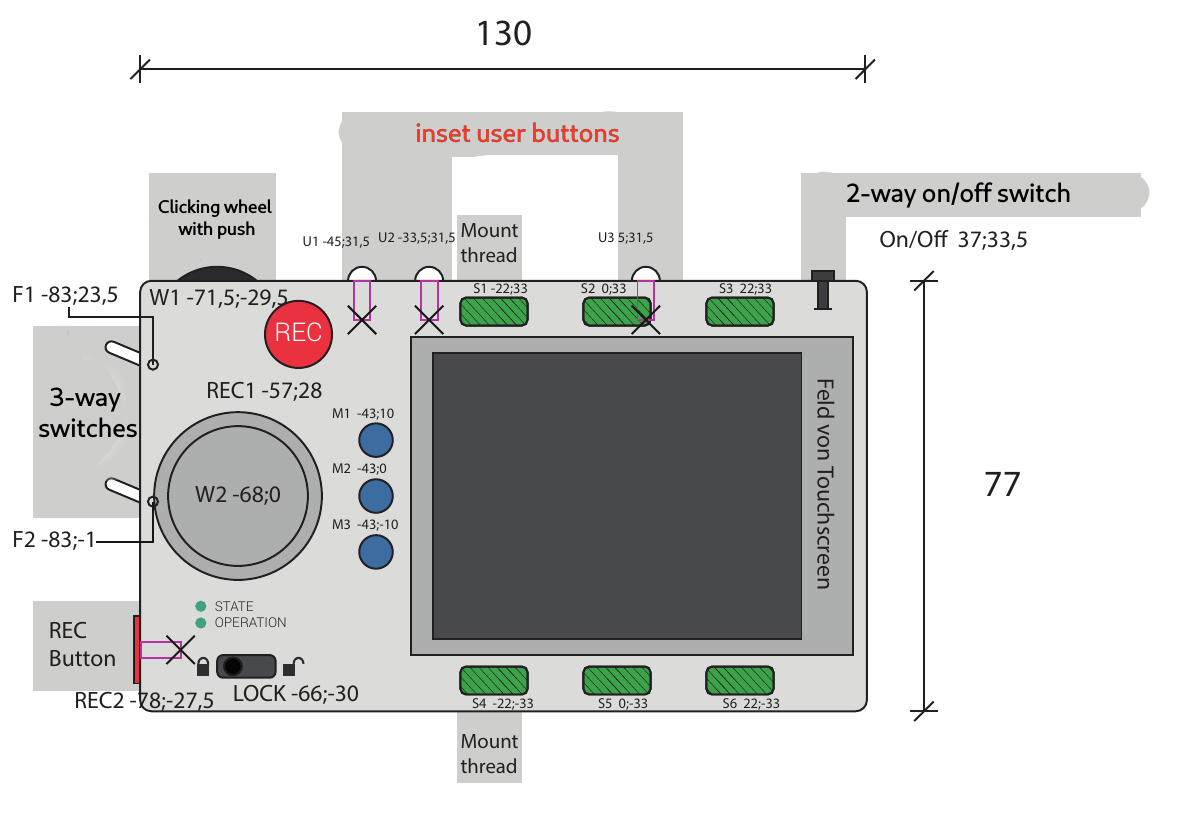
\includegraphics[width=0.8\linewidth]{images/axiom_remote_bottonPos.png}
		    \caption{AXIOM Remote Button Positions}
		    \label{fig:logo}
		\end{figure}
	\end{center}
\end{frame}

\subsection{Operation}

\begin{frame}{Operation}
	\begin{center}
		\begin{figure}[h]
		    \centering
		    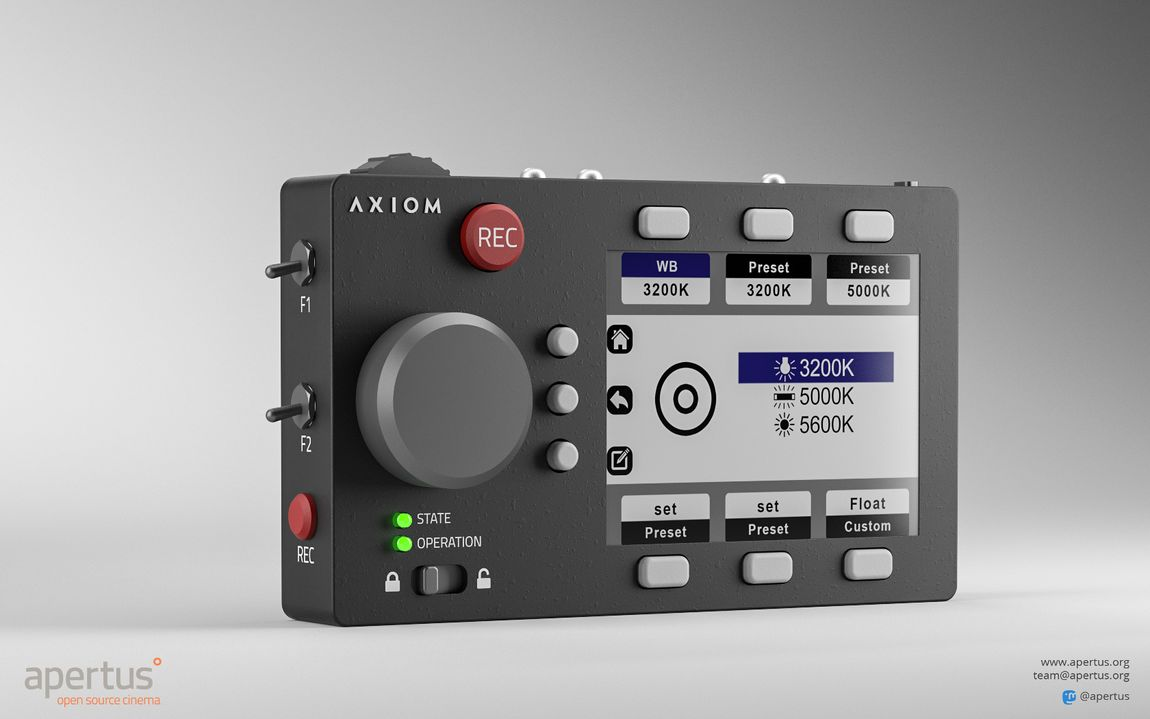
\includegraphics[width=0.8\linewidth]{images/Axiom_Remote_V3.jpg}
		    \caption{AXIOM Remote}
		    \label{fig:logo}
		\end{figure}
	\end{center}
\end{frame}


\begin{frame}{Operation (Cont.)}
	\begin{itemize}
		\item Six buttons - to select the options
		\item Currently in the new design - only "home" and "back" buttons are present
		\item In the older version - there are left/right buttons to change the pages, a page number button to goto a particular page and for the menu items which are not self-explanatory there is a "?" (help) button
	\end{itemize}
\end{frame}

\subsection{Hardware}

\begin{frame}{Hardware}
	\begin{itemize}
		\item PCB Version 2 Prototype
		\begin{itemize}
			\item The second knob is removed
			\item Remove left side rocker switches
			\item Remove top side pushbuttons
			\item Having one white LED per pushbutton
			\item 4 more holes to PCB
			\item Replace slide switches for ON/OFF and LOCK with pushbuttons
		\end{itemize}
	\end{itemize}
\end{frame}

\begin{frame}{Hardware (Cont.)}
	\begin{center}
		\begin{figure}[h]
		    \centering
		    \includegraphics[width=0.8\linewidth]{images/Axiom_Remote_PCB.jpg}
		    \caption{PCB}
		    \label{fig:logo}
		\end{figure}
	\end{center}
\end{frame}

\subsection{Electronics}

\begin{frame}{Electronics}
	\begin{itemize}
		\item PIC32MZ was chosen as core processor, two PIC16 are used for handling push button, rotary encoder and LED IO
		\item 2.8" 320x240 TFT from Adafruit as a display
		\item USB-C Connector
		\item Currently powered externally via 5V DC supply
		\item The firmware is programmed with a PICkit2 directly into the flash memory
	\end{itemize}
\end{frame}

\subsection{GUI}

\begin{frame}{GUI}
	\begin{center}
		\begin{figure}[h]
		    \centering
		    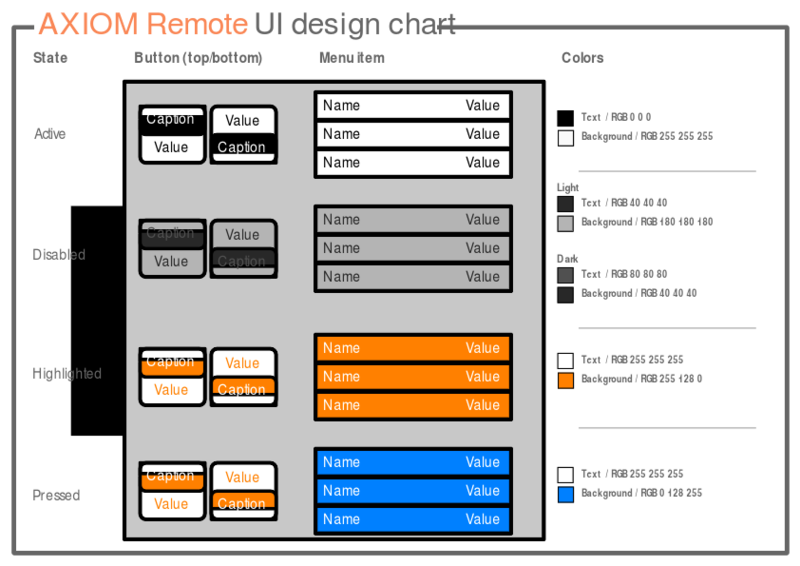
\includegraphics[width=0.8\linewidth]{images/AXIOM_Remote_UI_design_chart.png}
		    \caption{Color Scheme}
		    \label{fig:logo}
		\end{figure}
	\end{center}
\end{frame}

\end{document}
